\documentclass[a4paper,12pt]{article}
\usepackage{url}
\usepackage{listings}
\usepackage{color}
\usepackage{hyperref}
\usepackage{graphicx}
\usepackage{booktabs}
%\usepackage{mdframed}
\usepackage{adjustbox}

\definecolor{dkgreen}{rgb}{0,0.6,0}
\definecolor{gray}{rgb}{0.5,0.5,0.5}
\definecolor{mauve}{rgb}{0.58,0,0.82}

\lstset{frame=tb,
	language=C++,
	aboveskip=3mm,
	belowskip=3mm,
	showstringspaces=false,
	columns=flexible,
	basicstyle={\small\ttfamily},
	numbers=none,
	numberstyle=\tiny\color{gray},
	keywordstyle=\color{blue},
	commentstyle=\color{dkgreen},
	stringstyle=\color{mauve},
	breaklines=true,
	breakatwhitespace=true,
	tabsize=3
}
\begin{document}
	
	\title{CS-224 Object Oriented Programming and Design Methodologies }
	\author{Homework 03}
	\date{Fall 2022}
	\maketitle
	
	
	\section{Submission Policy}
	You need to submit this homework on  {\color{blue}07th October at 8pm}, on LMS. Late submissions are allowed until {\color{red} 09th October 11:59pm}, which will be penalized by 20\%. Your work will not be accepted once the submission is closed on LMS.
	

	\section{Guidelines}
	\begin{itemize}
		\item You need to do this assignment in a group of two students.
		\item You will submit your assignment to LMS (only one member of the group will submit).
		\item Clearly mention the group composition in submitted file name e.g. AhmadHassan\_ah01345\_BatoolAiman\_ba03451.zip. 
		\item You need to follow the best programming practices 
		\item Submit assignment on time; late submissions will not be accepted.
		\item Some assignments will require you to submit multiple files. Always Zip and send them.
		\item It is better to submit incomplete assignment than none at all.
		\item It is better to submit the work that you have done yourself than what you have plagiarized.
		\item It is strongly advised that you start working on the assignment the day you get it. Assignments WILL take time.
%		\item Every assignment you submit should be a single zipped file containing all the other files. Suppose your name is John Doe and your id is 0022 so the name of the submitted file should be JohnDoe0022.zip
		\item DO NOT send your assignment to your instructor, if you do, your assignment will get ZERO for not following clear instructions.
		\item You can be called in for Viva for any assignment that you submit
	\end{itemize}
	

	
	\section{Package Delivery System}
	For this assignment you will be implementing a \href{https://www.javatpoint.com/binary-search-tree}{binary search tree(BST)} composed of Truck variable. Truck structure is defined as:

	\begin{lstlisting}
		struct Truck
		{
		    string driver;
		    double petrol;
		    string regNo;
		    int fullMileage;
		    int emptyMileage;
		};
	\end{lstlisting}

You will be using the sample file, \path{Input.txt} for this assignment. Your code should however take into account that if an entry is increased or reduced (5 lines per entry) it reads all the entries in the file (You are going to assume that there are no errors in the file). For example, if there is just one entry:\smallskip\\
	
	\noindent Elton John\\
	34\\
	AB218\\
	9\\
	7\\
	
	

	\noindent Based on this entry, the driver's name is Elton John, the truck has 34 liters of petrol in its tank, its registration number is AB218. It covers 9 km per liter if empty and 7 km per liter when loaded.\\
	
	\noindent The function \texttt{loadTrucks()} reads the file \texttt{Input.txt}, and populates a BST of trucks according to information given in the file. You can compare a truck variable is less than other truck variable on the basis of its registration number, hence based on this comparison you can populate the binary search tree. As you read information of a truck, a new BSTNode is created and inserted in proper location in the BST. 
	
	\noindent The function \texttt{makeJourney()} traverses all the trucks and updates their remaining fuels after a truck takes cargo and travel 60 km, drop the cargo and return empty based on the fuel consumptions. For example, the truck information given above can make this journey, as it has 34 litres petrol in its tank and it requires  $60/9 + 60/7 = 15.23$ litre of petrol. Hence the remaining fuel in this truck would be 18.77 litre. Those trucks who are unable to make the journey will will not travel, and hence their fuel information will not be updated. \\


	\noindent Finally, the function \texttt{unloadTrucks()} shows all the trucks information in ascending order of registration number. A new file \path{Trip.txt} should be generated that will show the current state of all the Trucks. The file format is similar as Input.txt.\smallskip\\	

	Note: this question does not require SDL files.
	
	\section{HUMania}
	
A sample code is given in HUMania folder, if you run it you can see a pigeon is moving slightly towards right side. This example creates just one variable of  Unit type, and draws pigeon taken from assets file. 
	
You are required to create 3 different types of objects drawn on the screen: Pigeon, Butterfly and Bee. As you click on the screen the function createObject is called with mouse coordinates given in x, y variables. You have to create a pigeon, butterfly or a bee randomly on the screen. You'll be maintaining 3 different std::vectors (refer to section \ref{vectorTutorial}), one for each of the item drawn. Please refer to section \ref{sdlDrawing}, you only have to change srcRect to draw different type of items. 

Animations: As you draw the objects on screen, you also have to animate them. For this purpose, you cycle through the 3 different states of the object as given in assets file. 
All of the objects should keep moving slightly towards right, and when an object is reached to right most corner of the screen, it should reappear from the left most corner of the screen. 

%	 \begin{itemize}
%	 	\item Create a \texttt{Pigeon} class (see the pigeon.hpp/cpp), that will contain attributes and functions (\texttt{fly, draw}) related to a pigeon. The \texttt{fly} function flies the pigeon gradually to top-right side, and gets back the pigeon to left most corner as they approach at the right most border of the window. Three different images in assets file will be changed back and forth to make the pigeon fly. \texttt{draw} is only drawing the Pigeon object.
%	 	
%	 	\item Create an \texttt{Egg} class (create Egg.hpp and Egg.cpp), that will contain attributes and functions (\texttt{drop, draw}) related to egg. \texttt{drop} function makes the egg drop on the floor. Its shape changes to broken egg as it reaches to bottom of screen, and it doesn't move further down. \texttt{draw} function is only drawing the Egg object.
%	 	
%	 	\item Create a \texttt{Nest} class (create Nest.hpp and Nest.cpp), that will contain attributes and functions (\texttt{wiggle, draw}) related to Nest. \texttt{wiggle} is making a nest wiggle on the screen (without dropping down). Look at the three images in assets file to make a nest wiggle. \texttt{draw} function is only drawing the Nest object.
 

	\begin{figure}
		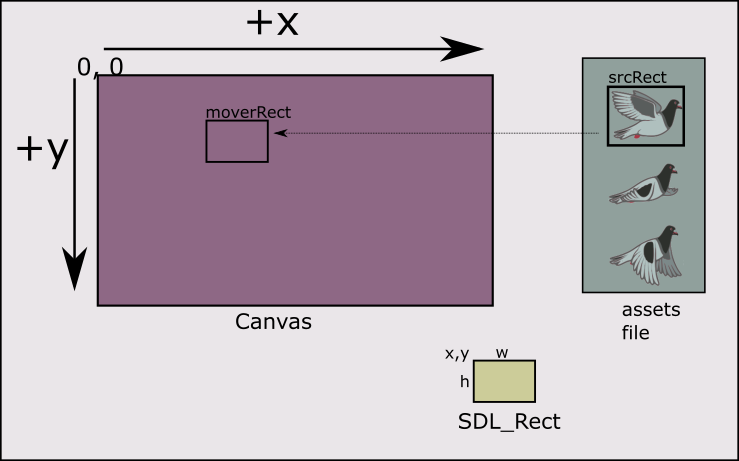
\includegraphics[width=\linewidth]{sdlDrawing}
		\caption{SDL Drawing Basics}
		\label{fig:sdlDrawing}
	\end{figure}  

	
	
	\subsection{SDL Drawing Basics}\label{sdlDrawing}
	
	The basic drawing function in SDL is very simple, you need two SDL\_Rect variables to draw a portion of image from assets file to the canvas. \texttt{SDL\_Rect} is a simple structure containing \texttt{\{x, y, w, h\} }attributes. \texttt{(x, y)} is the top-left corner, and \texttt{w, h} are width and height of rectangle. You define a \texttt{srcRect} for desired object in assets file, and define a \texttt{moverRect} for this image to be drawn on desired location on canvas. Refer to Figure \ref{fig:sdlDrawing} for all this process.  Finally you call 
	
	\noindent \texttt{SDL\_RenderCopy(gRenderer, assets, \&pigeonSrc, \&pigeonMover);}
	
	\noindent that displays this image to the canvas, voila!!!. Refer to \texttt{assets.png} file for all the required image assets.
	
	You can draw as many objects in the \texttt{HUMania.cpp $ \Rightarrow $ drawObjects()}, as you want. Since this function is called infinitely, you can change the \texttt{x, y} attributes of \texttt{moverRect} to move the objects on screen, and you can change the \texttt{srcRect} values to get a flying animation.
	


	\section{\texttt{std::vector} Tutorial} \label{vectorTutorial}
	
	Following is a basic example to work with vector. Complete reference for C++ vector is given here \url{https://en.cppreference.com/w/cpp/container/vector}
	\begin{lstlisting}
#include<iostream>
#include<vector>

using namespace std;

struct Distance{
	int feet, inches;
};

int main(){
	vector<Distance> dst; // It's a vector that can store Distance type objects
	dst.push_back(Distance{3, 4}); // create an object, and push it in vector
	dst.push_back(Distance{5, 2});
	dst.push_back(Distance{2, 7});
	dst.push_back(Distance{7, 8});
	dst.push_back(Distance{13, 1});

    Distance d1 = {5, 12}; 
    dst.push_back(d1);
	
	for(int i=0;i<dst.size();i++)
		cout<<dst[i].feet<<"'"<<dst[i].inches<<'"'<<endl; // call show method of dst[i] object
}

//////////////// Output: ///////////////////
3'4"
5'2"
2'7"
7'8"
13'1"
5'12"
	\end{lstlisting}
	
	\section{Some important points:} 
	
	\begin{itemize}
		\item Sample code is there for your benefit. If you are going to use it, understand how it works. 
		\item You do not need to follow the code given exactly. You can make changes where you see fit provided that it makes sense.
%		\item Make the class declarations in hpp files, and provide function implementations in cpp files. Don't use hpp files for implementation purposes.
%		\item Implement Q1 prior to implementing Q2, it will help you to implement linked list.
%		\item Where necessary, declare your own functions inside classes. Make sure why you would keep a function as private or public.
%		\item As a general rule, class's deta is private, and functions are public. Don't use getter/setter functions to manipulate data, rather think in object oriented directions and provide all the functionality in the class.
		\item Complete reference for C++ vector is given here \url{https://en.cppreference.com/w/cpp/container/vector}
		\item You need to define separate \path{*.hpp} and \path{*.cpp} files for all the classes.
		\item Exact x,y,w,h values for images in assets file can be found by \url{http://www.spritecow.com/}. 
		\item A tutorial for file I/O is given \url{http://www.cplusplus.com/doc/tutorial/files/}. 
		\item You should take \url{www.cplusplus.com} and \url{www.cppreference.com} as primary web source to search about C++
		\item You have to follow best OOP practices as discussed in lectures.
	\end{itemize}

\newpage

		\section{Rubric}
	\begin{table}[!h]
		\centering
		\begin{tabular}{llc}
			\toprule
			Warnings/Errors	& The code had no warnings/errors	& 1 \\
			Comments &	The code was properly commented	& 2 \\
			Coding	& The code followed best practices guideline &	2 \\
			OOP Concepts & The code followed best OOP practices & 5 \\
			% Modularization &	Code is modularized in different functions	& 1\\
			Functionality	& All the functionality is implemented as described above	& 10 \\
			\midrule
			Total & & 20\\
			\bottomrule
		\end{tabular}
		\caption{Grading Rubric}
		\label{Grading}
	\end{table}
	\section{Credits}
		Some questions in this assignment are derived from the work of Dr. Umair Azfar Khan.

	\newpage
	
	
\end{document}